\documentclass[11pt,a4paper]{article}
\usepackage[utf8]{inputenc}
\usepackage[T1]{fontenc}
\usepackage[english]{babel}
\usepackage{lmodern}
\usepackage[margin=2.5cm]{geometry}
\usepackage{graphicx}
\usepackage{booktabs}
\usepackage{longtable}
\usepackage{caption}
\usepackage{microtype}
\usepackage[hidelinks]{hyperref}
\captionsetup{font=small,labelfont=bf}
\setlength{\parskip}{0.4em}
\setlength{\parindent}{0pt}

\title{\textbf{Biopolymers, and the computational methods used to study them}\\[0.3em]
\large A bibliometric mapping of the field, with a Latin American and Colombian focus}
\author{Camila Argel \\ \small Directed by Aldo F. Combariza \\
\small Grupo de Investigación IN SILICO, Universidad de Sucre}
\date{Working draft, \today}

\begin{document}
\maketitle

\begin{abstract}
\noindent
This report maps the scientific literature on biopolymers and measures how much of it uses
computational chemistry, chemoinformatics or artificial intelligence. It then narrows to
Latin America and Colombia. The corpus is built from OpenAlex and cross-checked against
Lens, and the method layer is classified by reading abstracts rather than by matching
keywords. Two results shape everything that follows. Keyword bibliometrics overstates the
computational share of the field worldwide, because the vocabulary of biopolymers overlaps
that of structural biology; and it understates the share in Latin America, because much
regional work is invisible to affiliation matching. Reading the abstracts reverses the
ranking of contexts that the keyword counts produce.
\end{abstract}

\section{What this report answers}

Three questions, in the order the work addressed them.

\begin{enumerate}
\item Where and when is research on biopolymers being done, and by whom?
\item How much of that research uses computational chemistry, chemoinformatics or
      artificial intelligence, and which methods on which polymers?
\item What does the Latin American and Colombian position look like inside that map?
\end{enumerate}

The thematic scope is deliberately wide: every biopolymer recognised as a subject of
scientific study, anchored on the lines this group works in jointly, namely cellulose and
nanocellulose, polyhydroxyalkanoates, and lignin.

\section{Method}

\subsection{How the corpus was defined}

The core corpus is the field that \emph{identifies itself} as biopolymers: works whose
title or abstract carries a biopolymer framing term. This was reached empirically. Blocks
for each polymer family were probed first, and every family block intersected with a
biopolymer framing turned out to be a subset of the generic string, so the generic string is
the union rather than a narrowing.

Two acronym tests decided the wording of every query. The bare acronym PHA returns 56{,}015
records against 8{,}422 when bound to its expanded form, and bare DFT 471 against 295 inside
the core corpus. Bare acronyms are used nowhere.

Every search string is a versioned file that is never edited once run, so a count can always
be traced to the exact text that produced it.

\subsection{Sources}

Scopus and Web of Science are not used: the institution has no subscription. The
triangulation therefore runs on OpenAlex as the base corpus and Lens as an independent
index, with Semantic Scholar and Europe PMC recovering abstracts that OpenAlex lacks.

This turned out to be more informative than a comparison of two commercial indexes would
have been. Table~\ref{tab:sources} shows Lens holding most of the world corpus but a far
smaller share of the regional one.

\begin{table}[htbp]
\centering
\caption{OpenAlex against Lens, same concept, same window. Lens covers the world corpus
well and the regional corpora poorly, so the choice of source matters most exactly where
this report focuses.}
\label{tab:sources}
\small
\begin{tabular}{llrrr}
\toprule
Block & Region & OpenAlex & Lens & Lens as \% of OpenAlex \\
\midrule
Core field & World & 142,254 & 129,729 & 91.2 \\
Core field & Latin America & 8,147 & 5,412 & 66.4 \\
Core field & Colombia & 598 & 342 & 57.2 \\
Method layer & World & 3,912 & 3,323 & 84.9 \\
Method layer & Latin America & 211 & 104 & 49.3 \\
Method layer & Colombia & 17 & 4 & 23.5 \\
Cellulose & Latin America & 14,222 & 9,813 & 69.0 \\
Cellulose & Colombia & 897 & 558 & 62.2 \\
PHA/PHB & World & 22,225 & 20,241 & 91.1 \\
PHA/PHB & Latin America & 1,444 & 1,037 & 71.8 \\
PHA/PHB & Colombia & 88 & 64 & 72.7 \\
Lignin & Latin America & 11,464 & 8,598 & 75.0 \\
Lignin & Colombia & 810 & 635 & 78.4 \\
\bottomrule
\end{tabular}
\end{table}

The overlap is partial in both directions. Across the matched corpora, between 76\% and 100\% of Lens records are also in OpenAlex, but only between 24\% and 75\% of OpenAlex records are in Lens. Lens still contributes works OpenAlex
lacks, so the union of the two is larger than either. A single-source count of Latin
American output is therefore a lower bound, and this is a result rather than a caveat.


\subsection{Reading the abstracts}

A keyword query cannot tell a molecular dynamics study of a cellulose nanocrystal composite
from a molecular dynamics study of haemoglobin allostery, yet only the first is biopolymer
materials science. Every abstract in the method layer was therefore classified by a language
model: whether the work is materials research or biological-function research, which polymer
family, which computational method, and whether experiments are reported. Every call is
cached on a hash of the prompt, so the classification is reproducible and re-running it is
free.

One correction was applied after inspecting the output rather than trusting it. The first
pass offered a catch-all computational category, and it was absorbing factorial designs,
response-surface methodology and curve fitting to the authors' own measurements. That
inflated the Colombian computational share to 12.5\% against a defensible 3\%. The ambiguous
bucket alone was re-asked with a question naming the distinction, and statistical design of
experiments is now excluded from every computational count. The first-pass classifications
are kept on disk so the correction is auditable.

\subsection{Validating the screening}
\label{sec:validation}

A classification produced by a language model is worth nothing without an agreement figure.
125 abstracts were double-coded by a second, independent reader on a different model,
blind to the first coder's labels. Asking the same model to check its own work would have
it repeat its own mistakes and report high agreement with itself.

Agreement is reported as Cohen's kappa rather than percent agreement, because percent
agreement flatters any classification with a dominant class.


\begin{table}[htbp]
\centering
\caption{Agreement between the two independent coders on the random sample.}
\label{tab:validation}
\small
\begin{tabular}{lrr}
\toprule
Dimension & Agreement & Cohen's $\kappa$ \\
\midrule
materials vs biological & 94.0\% & 0.878 \\
computational at all & 92.0\% & 0.782 \\
method family & 88.0\% & 0.816 \\
polymer family & 80.0\% & 0.767 \\
\bottomrule
\end{tabular}
\end{table}


The distinction the whole correction depends on, materials research against biological
function, reaches the highest agreement of the four. On the conventional reading, 0.61--0.80
is substantial and above 0.80 almost perfect.

The two coders also disagree in a consistent direction. On the random sample of 100, the
first coder called 79 works computational against the second coder's 73, a relative
over-detection of 8.2\%. Five of the seven disputed works were labelled machine learning,
and reading them shows why: they are reviews and experimental papers that mention artificial
intelligence as a closing perspective without performing any computation. \\textbf{Every
screened share in this report is therefore an upper bound}, and the strict world figure of
1.28\%
is closer to 1.18\% once the bias is applied. This runs the same way as every other
correction found here.

\section{Results}

\subsection{Size, growth and geography}

\begin{table}[htbp]
\centering
\caption{The field by context. Growth rates use complete years only. The method share here
is the \emph{keyword} estimate, corrected in Section~\ref{sec:layer}.}
\label{tab:contexts}
\small
\begin{tabular}{lrrrrr}
\toprule
Context & Works, all years & 2015--2025 & Share of world & Growth/yr & Open access \\
\midrule
World & 145,743 & 90,931 & 100.00\% & 11.4\% & 43.2\% \\
Ibero-America & 13,095 & 9,445 & 10.39\% & 13.7\% & 58.5\% \\
Latin America & 8,162 & 6,035 & 6.64\% & 14.7\% & 55.5\% \\
Colombia & 598 & 465 & 0.51\% & 27.0\% & 66.7\% \\
\bottomrule
\end{tabular}
\end{table}

The field holds 145,743 works and grows at 11.4\% a year. Both
regional contexts grow faster than the world, Latin America at 14.7\% and
Colombia at 27.0\%, so the region is closing the relative gap rather than
falling behind. Colombia's rate is computed on a small base and says more about the base
than about capacity. Regional output is markedly more open: 66.7\% of Colombian
work is open access against 43.2\% worldwide.

\begin{figure}[htbp]
\centering
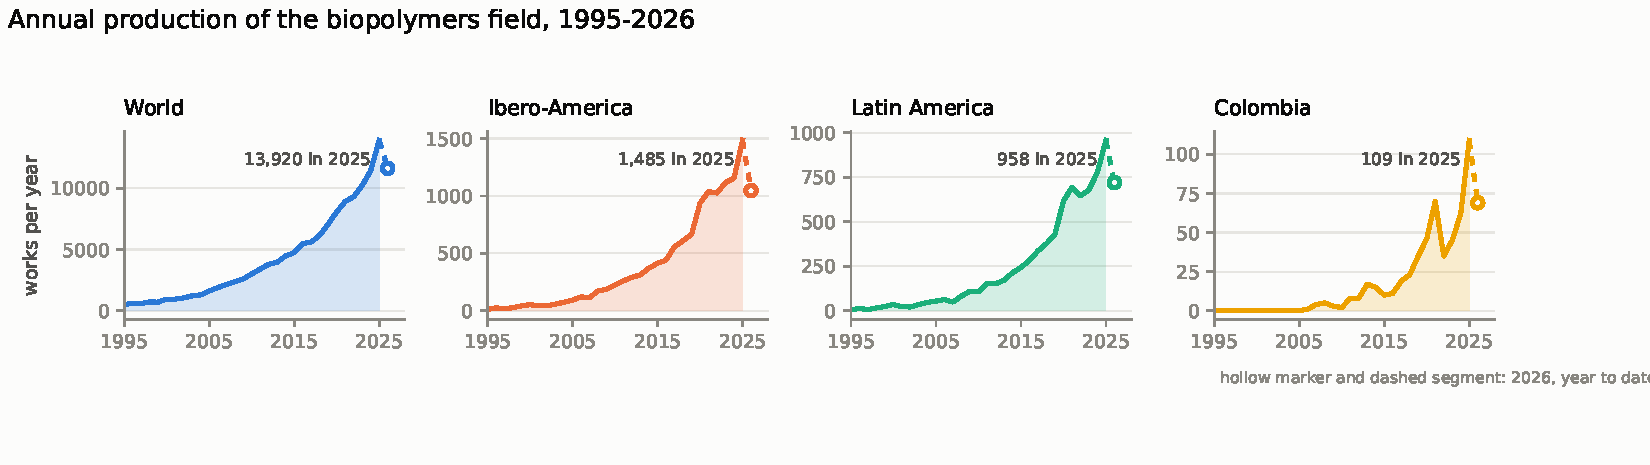
\includegraphics[width=\textwidth]{../outputs/figures/F1_annual_production.pdf}
\caption{Annual production by context. Each panel carries its own scale, since the contexts
differ by three orders of magnitude. The hollow marker and dashed segment are 2026, a
partial year.}
\end{figure}

The top three countries, United States, China and
India, hold 50,777 works between them, just over a third of the
field. Only one Latin American country reaches the top twenty:
Brazil.


Inside Latin America the order by volume is Brazil (4,450), Mexico (1,559), Argentina (794), Colombia (598), Chile (492), Ecuador (232).

\begin{figure}[htbp]
\centering
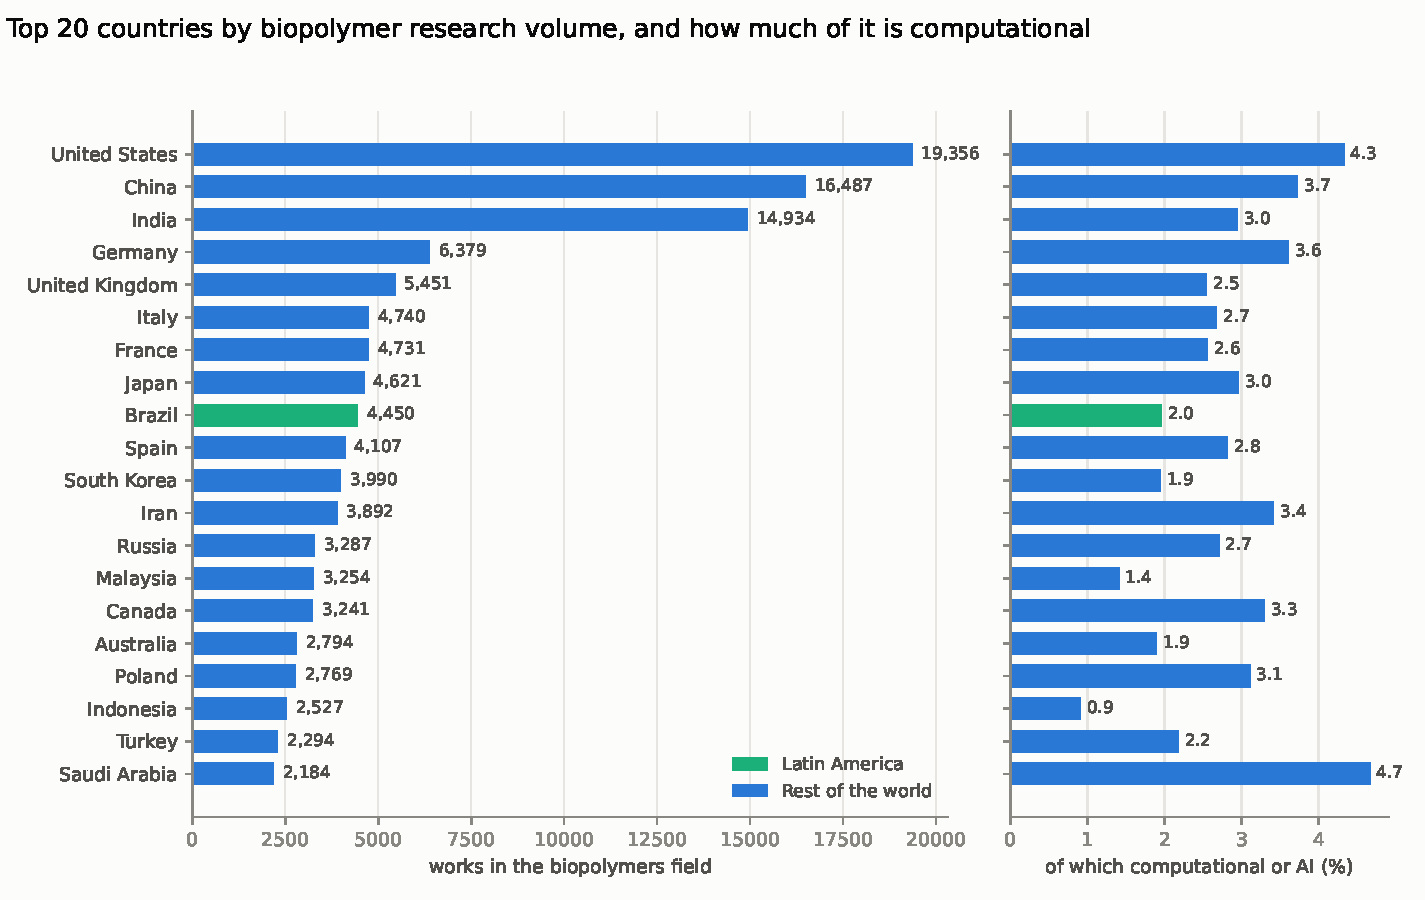
\includegraphics[width=\textwidth]{../outputs/figures/F3_country_ranking.pdf}
\caption{The twenty largest producers, and how much of each country's output is
computational. Volume and intensity are separate panels; they are different measures and do
not share an axis.}
\end{figure}

\subsection{The computational and artificial-intelligence layer}
\label{sec:layer}


This is the central result. The keyword estimate puts
2.63\% of the field on some computational, chemoinformatic or
AI method. Reading the abstracts shows only
56.6\% of that layer to be biopolymer
materials research; the rest is protein folding, enzyme mechanism and nucleic-acid biology,
pulled in because the framing terms overlap. Restricting to materials research brings the
share to 1.49\%, and restricting further to works
with a genuine computational method gives
\textbf{1.28\%}.

\begin{figure}[htbp]
\centering
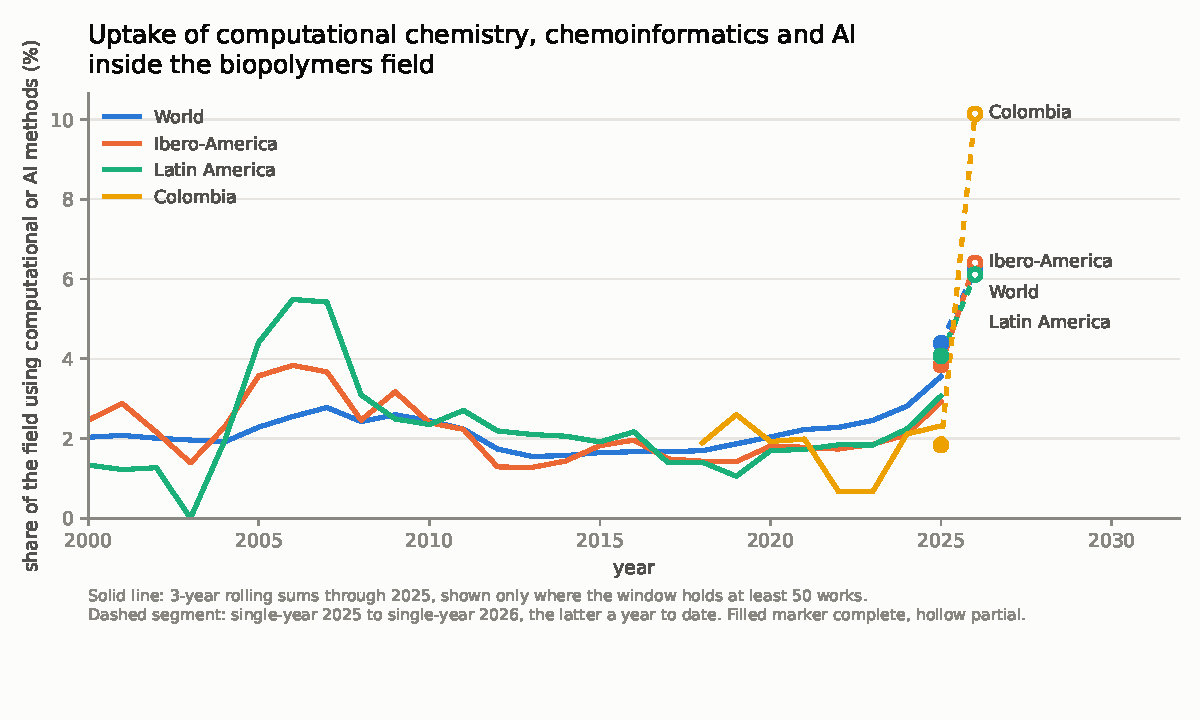
\includegraphics[width=0.92\textwidth]{../outputs/figures/F2_methods_share.pdf}
\caption{Uptake of computational methods inside the field. The solid line is a three-year
rolling share; the dashed segment joins single-year 2025 to single-year 2026, the latter a
year to date. Ratios on small denominators are suppressed.}
\end{figure}

\paragraph{The partial year is not dropped.} 2026 is incomplete and is kept, flagged,
because it carries the strongest signal in the data.

\begin{table}[htbp]
\centering
\caption{2026 to date against the whole of 2025. The field as a whole is well short of its
2025 volume at the same date, while the method layer has already passed it in every
context.}
\label{tab:partial}
\small
\begin{tabular}{lrrrrrr}
\toprule
& \multicolumn{3}{c}{Whole field} & \multicolumn{3}{c}{Method layer} \\
\cmidrule(lr){2-4}\cmidrule(lr){5-7}
Context & 2025 & 2026 YTD & \% & 2025 & 2026 YTD & \% \\
\midrule
World & 13,920 & 11,629 & 84 & 610 & 722 & 118 \\
Ibero-America & 1,485 & 1,046 & 70 & 57 & 67 & 118 \\
Latin America & 958 & 720 & 75 & 39 & 44 & 113 \\
Colombia & 109 & 69 & 63 & 2 & 7 & 350 \\
\bottomrule
\end{tabular}
\end{table}

\subsection{Keyword counts understate the region}

\begin{table}[htbp]
\centering
\caption{Screening the whole regional field, rather than the keyword-selected method layer,
finds computational work the query missed.}
\label{tab:regional}
\small
\begin{tabular}{lrrrr}
\toprule
Corpus & Materials works & With a method & Screened share & Keyword share \\
\midrule
Colombia, whole field & 446 & 20 & 4.48\% & 1.94\% \\
Latin America, whole field & 5,751 & 197 & 3.43\% & 2.20\% \\
\bottomrule
\end{tabular}
\end{table}

Reading abstracts raises the regional estimate substantially, and it changes the ordering:
Colombia sits \emph{above} the Latin American average, not below it as the keyword counts
say. The keyword-based ordering should not be quoted.


Part of the reason is mechanical. In the world method corpus,
12.7\% of authorships match no institution entity
at all, so the country they belong to receives no credit. A 2025 paper with two Peruvian
affiliations and one Mexican one counts, in the data, as Mexican alone. Since every regional
corpus here was selected on institution country, works whose regional affiliations all went
unmatched never entered it. Per-country loss is worst for the smallest producers. The
regional counts in this report are a lower bound.


\subsection{Which methods, on which polymers}

\begin{table}[htbp]
\centering
\caption{Method mix of the materials-only subset, as a percentage of each context. The
world leans on molecular dynamics; the region leans on machine learning and quantum
chemistry.}
\label{tab:methods}
\small
\begin{tabular}{lrrrr}
\toprule
Method & World & Ibero-America & Latin America & Colombia \\
\midrule
Molecular dynamics & 33.0 & 28.2 & 24.2 & 22.2 \\
Machine learning & 24.8 & 27.5 & 29.3 & 22.2 \\
Quantum chemistry & 16.5 & 22.8 & 24.2 & 33.3 \\
Docking & 5.7 & 4.7 & 4.0 & 0.0 \\
Solubility modelling & 3.5 & 2.0 & 0.0 & 0.0 \\
QSAR / QSPR & 1.4 & 0.0 & 0.0 & 0.0 \\
Generative & 0.6 & 0.0 & 0.0 & 0.0 \\
Other molecular modelling & 0.7 & 2.0 & 3.0 & 11.1 \\
Other informatics & 0.2 & 0.7 & 1.0 & 0.0 \\
Statistical design of experiments & 0.2 & 0.0 & 0.0 & 0.0 \\
None detected & 13.4 & 12.1 & 14.1 & 11.1 \\
\bottomrule
\end{tabular}
\end{table}

Generative methods and QSAR are absent from the region entirely, and worldwide the
generative slice is a handful of works. That is the emptiest part of the map and the most
obvious opening.

\subsection{The regional deficit is partly linguistic}
\label{sec:language}

Every count so far came from English queries. Spanish and Portuguese term variants were run
against the same regional slices and the set difference taken, so what is reported is not
how many records the Spanish and Portuguese strings return but how many they return that
the English string does \emph{not}.


\begin{table}[htbp]
\centering
\caption{What Spanish and Portuguese terms add. The last column is the set difference:
records the Spanish and Portuguese strings return that the English string does not.}
\label{tab:language}
\small
\begin{tabular}{llrrr}
\toprule
Block & Region & English & Spanish/Portuguese & Added \\
\midrule
Core field & Latin America & 8,159 & 1,364 & 1,252 (+15.3\%) \\
Core field & Colombia & 598 & 183 & 157 (+26.2\%) \\
Cellulose & Latin America & 14,669 & 4,218 & 3,952 (+26.9\%) \\
Cellulose & Colombia & 902 & 303 & 281 (+31.1\%) \\
PHA/PHB & Latin America & 1,444 & 221 & 199 (+13.8\%) \\
PHA/PHB & Colombia & 88 & 36 & 30 (+34.1\%) \\
Lignin & Latin America & 11,527 & 1,815 & 1,686 (+14.6\%) \\
Lignin & Colombia & 811 & 158 & 145 (+17.9\%) \\
\bottomrule
\end{tabular}
\end{table}


The addition is substantial and it is largest for Colombia. A bibliometric count of Latin
American biopolymer research built on English terms alone misses between a seventh and a
third of the corpus, depending on the slice. Taken with the affiliation-matching loss of
Section~\ref{sec:layer}, the regional figures in this report understate the region twice
over, for two independent and separately measurable reasons.

\subsection{The three anchored lines}

\begin{table}[htbp]
\centering
\caption{The biopolymer lines this group works in jointly.}
\label{tab:anchors}
\small
\begin{tabular}{lrrrrr}
\toprule
Line & World & Latin America & Colombia & Computational, world & Computational, region \\
\midrule
Cellulose and nanocellulose & 378,840 & 14,683 & 902 & 1.64\% & 1.69\% \\
PHA / PHB & 22,378 & 1,444 & 88 & 1.30\% & 1.52\% \\
Lignin & 181,260 & 11,534 & 811 & 2.08\% & 1.86\% \\
\bottomrule
\end{tabular}
\end{table}

Lignin is the most computationally studied of the three and PHA the least. Latin America
holds a larger share of world output in PHA and lignin than in cellulose, which fits a
region working from agro-industrial residues.

\begin{figure}[htbp]
\centering
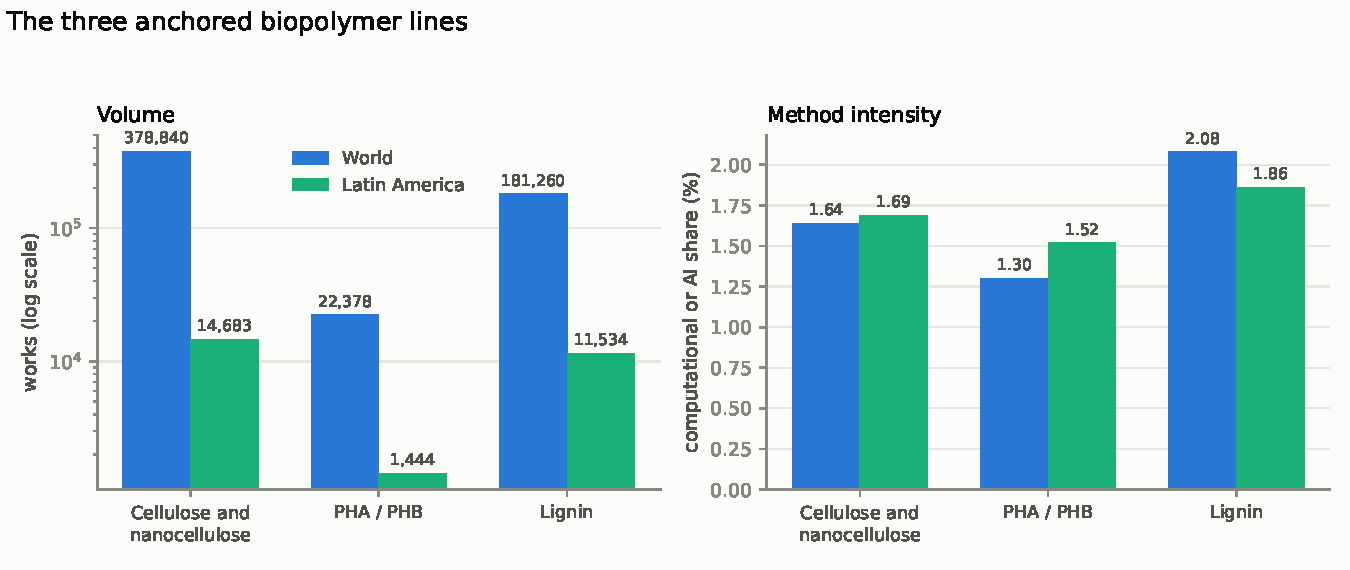
\includegraphics[width=\textwidth]{../outputs/figures/F4_anchor_lines.pdf}
\caption{Volume and method intensity of the three anchored lines.}
\end{figure}

\subsection{The generative frontier, read work by work}
\label{sec:generative}

The screening put ten works in the materials subset on generative or large-language-model
methods. Ten is few enough to read every one, and a count cannot say what these works
generate, what steers the generation, or whether anything is validated. Both coders read
all ten independently. Three disagreements followed, and all three change the answer.

\paragraph{Ten records are nine works.} A preprint on retrieval-augmented generation over
polyhydroxyalkanoate literature is indexed twice, once with a DOI and once without. The
automated pass counted both.

\paragraph{The lignin paper is not a large-language-model paper.} It trains autoregressive
\emph{molecular} language models on SMILES strings, which is a generative sequence model
over chemical structure rather than a language model over natural language. The confusion
is understandable and it moves the most methodologically serious work in the set into the
wrong category.

\paragraph{Three of the ten sit in venues that are not what they appear to be.} Two are
published as \emph{Frontiers in Agriculture} and \emph{Frontiers in Chemistry Materials
and Catalysis}, under DOI prefix 10.71465, which Crossref registers to \emph{International
Study Counselor}. Frontiers Media SA is 10.3389. A third carries prefix 10.37591,
registered to a different publisher again. All three abstracts share a pattern: dramatic
headline numbers with no dataset, no baseline and no reproducible protocol. No automated
screening asked about venue provenance, and none routinely does.


\begin{table}[htbp]
\centering
\caption{The generative works, as the two readers agreed them. ``Specific'' marks work
genuinely about a biopolymer rather than about polymers in general.}
\label{tab:generative}
\small
\begin{tabular}{rp{5.6cm}p{3.5cm}ll}
\toprule
Year & What it generates & Validated by & Specific \\
\midrule
2,026 & candidate biodegradable polymer formulations & experiment & yes \\
2,026 & candidate biodegradable polymer molecular structures & held out data & yes \\
2,026 & answers about polymer literature & none stated & yes \\
2,026 & candidate polymer repeat units & held out data & no \\
2,026 & polydisperse lignin molecular structures and simulation systems & simulation & yes \\
2,025 & biodegradable polymer structures for food packaging & simulation & yes \\
2,025 & candidate material compositions and microstructures & none stated & no \\
2,025 & 3D atomic polymer structures from repeat unit chemistry & held out data & no \\
2,021 & novel HFNAP polymer sequences & experiment & yes \\
\bottomrule
\end{tabular}
\end{table}


\paragraph{What survives.} Removing the works that are not about biopolymers and those
whose venue cannot be trusted leaves \textbf{four credible biopolymer-specific generative
works}, three of them from 2026. Two validated against the physical world, one by
electrospinning and mechanical testing, one by measuring nanomolar binding affinities. The
electrospun result was honestly negative: the fibre mat was weaker than commercial PET.

That is emptier than a count of ten suggests, and it strengthens the argument of this
report rather than weakening it. It also suggests that venue provenance deserves to be
checked across the whole corpus, not only on a shortlist, which nothing in the bibliometric
literature routinely does.

\subsection{Collaboration and community structure}

\begin{table}[htbp]
\centering
\caption{Collaboration, counted per work.}
\label{tab:collab}
\small
\begin{tabular}{lrrr}
\toprule
Corpus & Works & International & Two or more Latin American countries \\
\midrule
World, method layer & 3,328 & 30.4\% & 0.6\% \\
Latin America, whole field & 8,175 & 34.4\% & 6.0\% \\
Colombia, whole field & 598 & 44.1\% & 23.9\% \\
Latin America, method layer & 211 & 45.5\% & 9.0\% \\
\bottomrule
\end{tabular}
\end{table}

Colombia is the most regionally connected corpus measured. Nearly
24\% of Colombian works involve a second Latin American country, against
6\% for the region as a whole. Brazil's strongest ties run outward instead,
to the United States, Portugal and Spain, and dwarf its ties inside the region.

\begin{figure}[htbp]
\centering
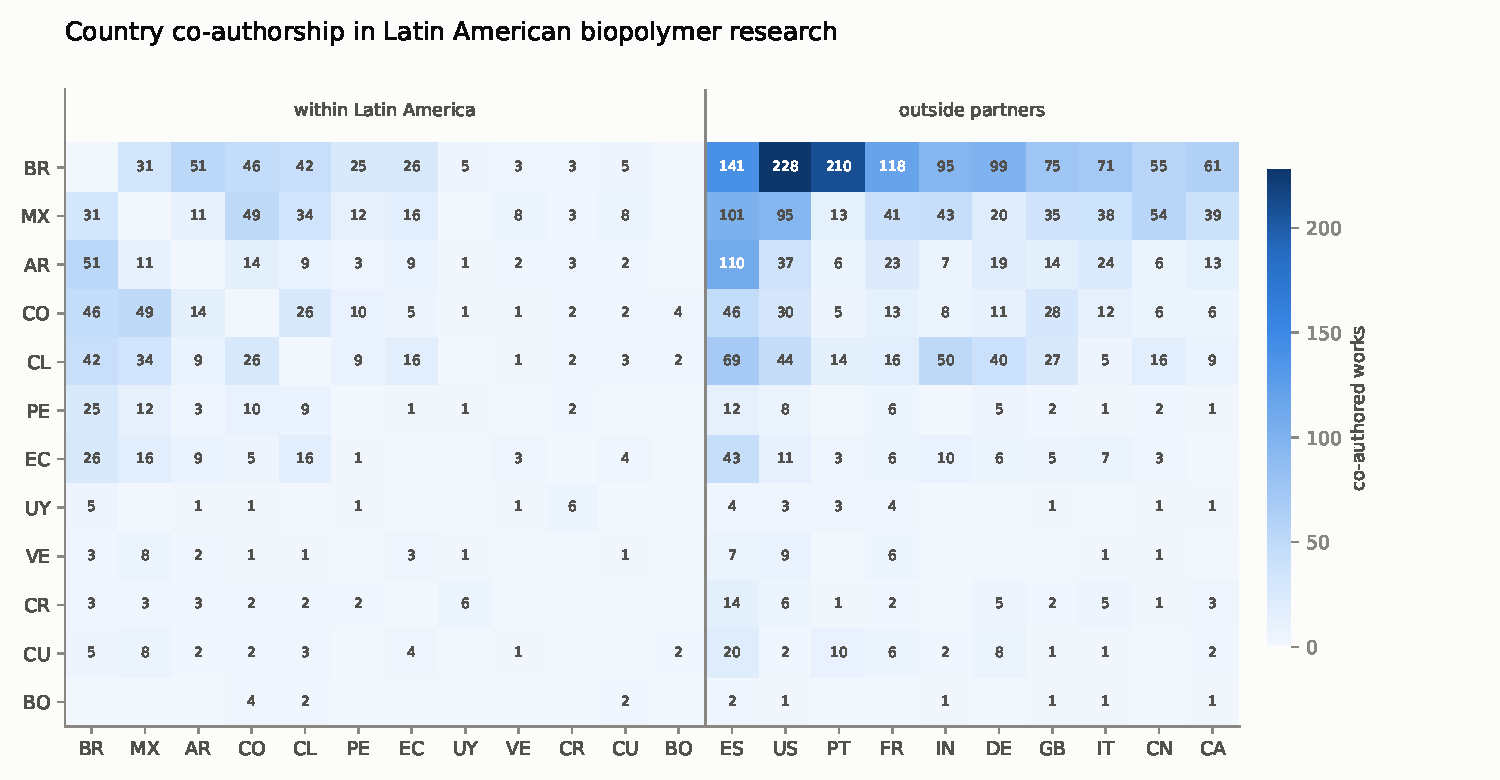
\includegraphics[width=\textwidth]{../outputs/figures/F5_collaboration_matrix.pdf}
\caption{Country co-authorship in Latin American biopolymer research, shown as a matrix. A
node-link drawing of the same 115-node graph is a hairball; the network files are provided
for VOSviewer instead.}
\end{figure}

\paragraph{There is no standing computational community.} Classic Lotka behaviour gives an
exponent near 2. Every corpus here is steeper, and the method layers are steepest of all: of
the 14,861 authors in the world method layer, 86.3\% appear exactly once, with a
fitted exponent of 3.46. The layer is made of one-off contributions. That is what a
field looks like before a speciality forms, not after.

\begin{figure}[htbp]
\centering
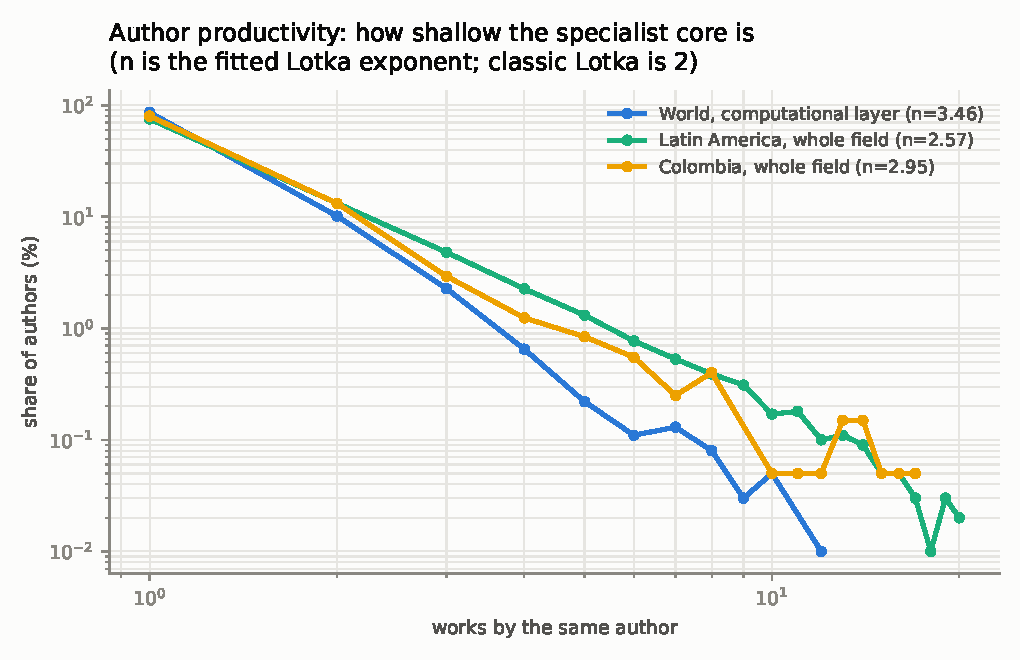
\includegraphics[width=0.85\textwidth]{../outputs/figures/F6_lotka.pdf}
\caption{Author productivity. A steeper slope means a shallower core of specialists.}
\end{figure}

\paragraph{And it has no home venue.} Bradford's core zone is the set of journals carrying
the first third of a corpus. Worldwide it is 2.4\% of journals, which is normal. For
the Latin American method layer it takes 13.2\% of its journals to reach the first
third. That work is scattered, with no venue acting as a centre.


\subsection{Colombia}

The Colombian institutional ranking is led by Universidad Nacional de Colombia (96), Universidad del Valle (66), University of Cartagena (47), Universidad de Antioquia (47). Universidad de Sucre appears with 25 works.

\begin{figure}[htbp]
\centering
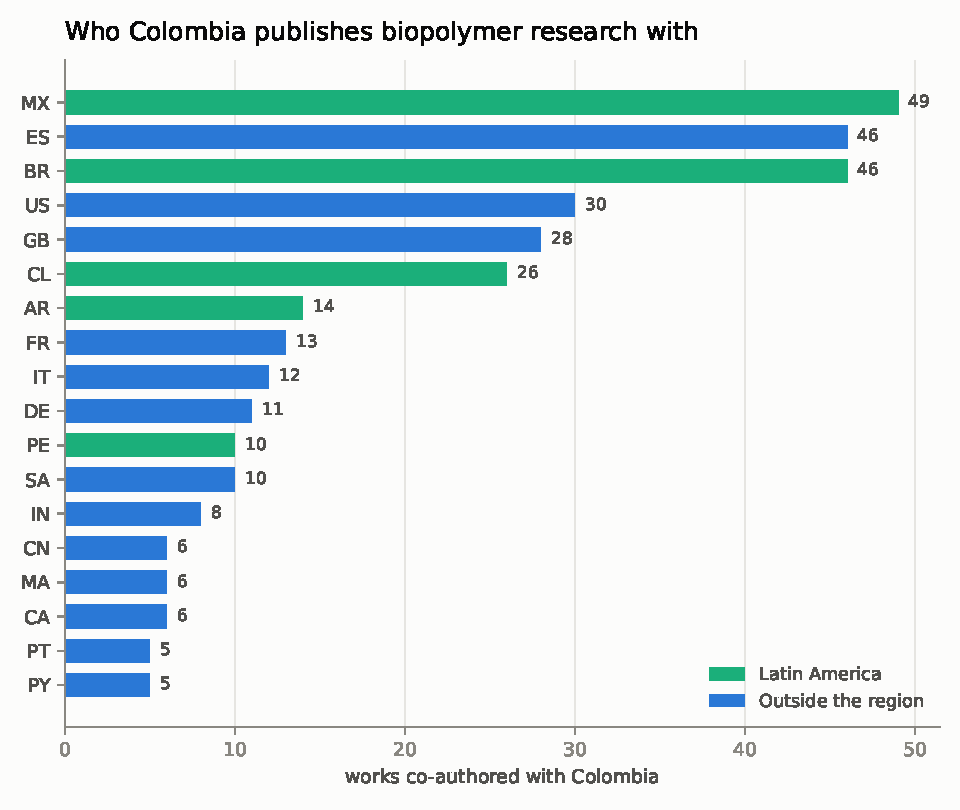
\includegraphics[width=0.8\textwidth]{../outputs/figures/F7_colombia_partners.pdf}
\caption{Colombia's co-authorship partners, split between the region and outside it.}
\end{figure}

\section{What the map shows}

\begin{enumerate}
\item \textbf{The computational layer is thin and it is accelerating.} Around one work in
      eighty in the biopolymers field uses a genuine computational method on a material.
      That share roughly doubled over a decade and 2026 is running ahead of 2025 in every
      context measured.
\item \textbf{The regional deficit is volume, not method.} Latin America and Colombia adopt
      computational methods at rates comparable to, and by the screened measure above, the
      world. What the region lacks is scale and continuity of output, not access to
      computational practice. This reverses the usual framing and it changes what a
      recommendation should say.
\item \textbf{The method mix differs by region.} The world leans on molecular dynamics;
      Latin America leans on machine learning; Colombia leans on quantum chemistry. An
      infrastructural reading is available, since sustained dynamics needs computing time
      that the other two need less of, but the Colombian denominator is small and this
      belongs in the discussion as a hypothesis rather than in the results as a finding.
\item \textbf{Generative methods are essentially absent}, worldwide and entirely so in the
      region. Reading all of them one by one (Section~\ref{sec:generative}) leaves four
      credible biopolymer-specific works in the world literature. Of everything in this
      report, that is the clearest opening.
\item \textbf{There is no community and no venue.} Most authors in the computational layer
      publish there once, and the regional slice has no core journals. A thesis that wants
      to change something has a structural target, not only a topical one.
\end{enumerate}

\section{Limitations}

\begin{itemize}
\item \textbf{Two sources, not four.} Scopus and Web of Science were unavailable. OpenAlex
      and Lens disagree by about a third on regional counts, which bounds how precise any
      regional figure here can be.
\item \textbf{The screened shares are upper bounds.} The measured over-detection of
      Section~\ref{sec:validation} is 8.2\%, and it is not corrected in the tables, only
      stated. Read every screened percentage as a ceiling.
\item \textbf{English-only counts understate the region} by between a seventh and a
      third, measured in Section~\ref{sec:language}. The headline tables have not been
      rebuilt on the combined vocabulary; that is the next harvest, not a completed one.
\item \textbf{Affiliation matching loses regional work.} Quantified in
      Section~\ref{sec:layer}. The regional counts are a lower bound.
\item \textbf{Abstract coverage.} Roughly 30\% of the method-layer records carry no abstract
      in OpenAlex. Semantic Scholar and Europe PMC recovered 4{,}070 of them; the rest could
      not be read and are excluded from every screened share.
\item \textbf{The screening is not yet validated.} A hand-coded sample double-coded against
      the automatic classification would give an agreement figure. Until that exists, the
      screened shares should be reported as what they are, a machine reading.
\item \textbf{English-language queries.} Regional work published in Spanish and Portuguese
      is undercounted.
\item \textbf{Country attribution counts a work once per country present}, so country
      columns sum to more than the corpus.
\end{itemize}

\section{What to do next}

\begin{enumerate}
\item A third coding of a few dozen items by a domain expert, as a check on two automatic
      coders that may share a bias neither detects.
\item Rebuild the headline corpus on the combined English, Spanish and Portuguese
      vocabulary, now that the addition has been measured.
\item Apply the venue-provenance check of Section~\ref{sec:generative} to the whole
      corpus. It is a measurable, publishable statement and nothing in the field does it.
\item Take the affiliation-matching loss seriously as a result in its own right. It is a
      measurable, publishable statement about how invisible small Latin American
      institutions are to the infrastructure that counts science.
\end{enumerate}

\vfill
\noindent\rule{\textwidth}{0.4pt}\\
\footnotesize
Every number in this report is generated from the analysis tables in
\texttt{outputs/tables/} by \texttt{scripts/python/build\_report.py}; none is typed by hand.
Search strings are versioned in \texttt{queries/}, the session record is in
\texttt{docs/LOG.md}.

\end{document}
